\documentclass[UTF8,a4paper]{paper}
\usepackage{ctex}
\usepackage[utf8]{inputenc}
\usepackage{amsmath}
\usepackage{pdfpages}
\usepackage{graphicx}
\usepackage{wrapfig}
\usepackage{listings}
\usepackage{multicol}
\usepackage{float}
\newcommand{\tabincell}[2]{\begin{tabular}{@{}#1@{}}#2\end{tabular}}
\title{实验四\ \ 波形发生电路仿真及实验}
\author{张蔚桐\ 2015011493\ 自55}
\begin {document}
\maketitle
\section{仿真和预习}
\subsection{正弦波发生电路}
\subsubsection{理论计算}
\begin{multicols}{2}
如图\ref{ACCirc}所示是正弦波发生电路的电路图,运放引入负反馈分析,如果使$R_1=R_2=R,C_1=C_2=C$,则可以得到选频网络得到的频率是
$$f_0=\frac{1}{2\pi RC}$$
因此如果要求$f_0=400Hz$,计算得到$R=12\mathrm{k}\Omega,C=33,000\mathrm{pF}(333)$,同时经过进一步的计算可以估计输出电阻的值基本令人满意。
\begin {figure}[H]
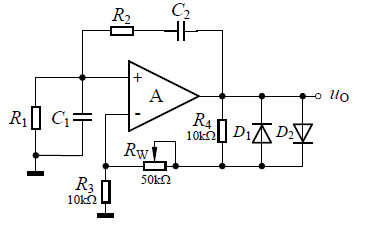
\includegraphics [width=\columnwidth]{ac.png}
\caption{正弦波发生电路}
\label{ACCirc}
\end {figure}
\end{multicols}
\subsubsection{输出波形调试}
\begin {figure}
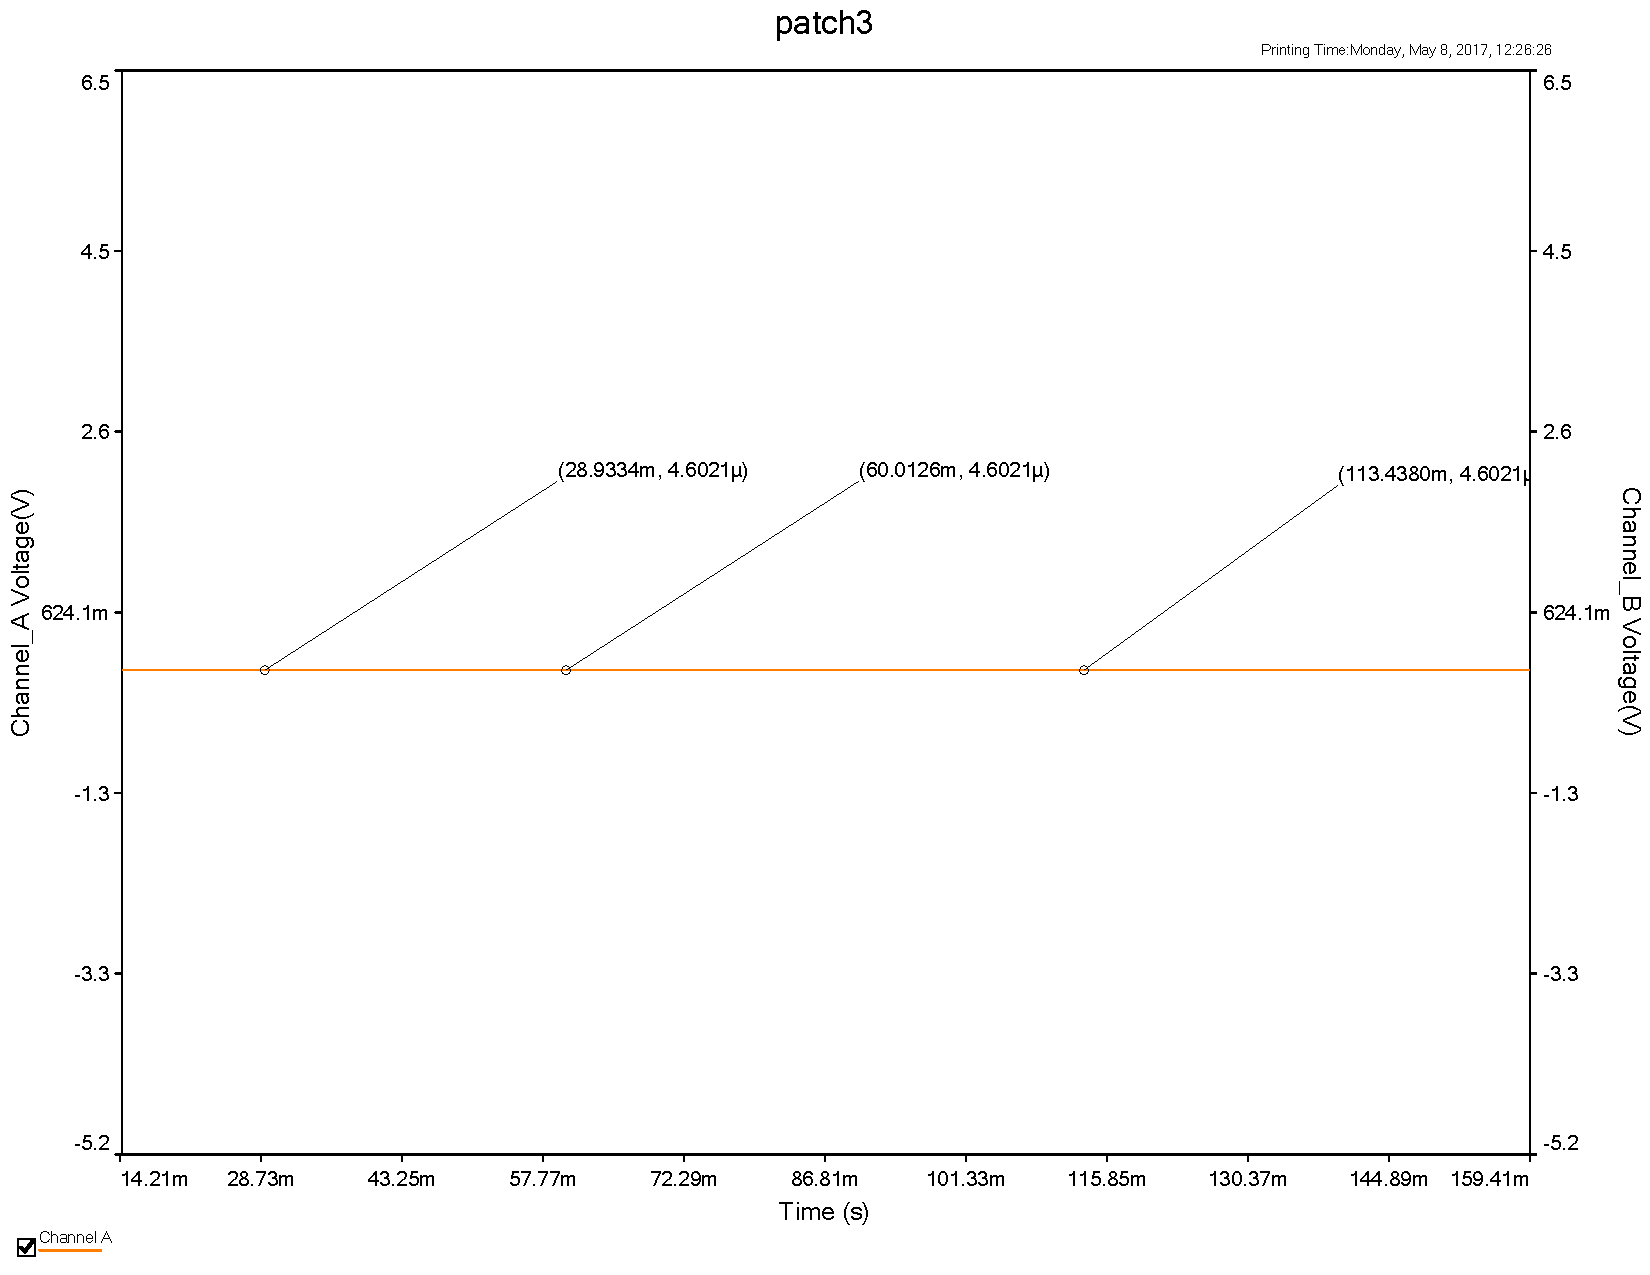
\includegraphics [width=\textwidth]{0ac.pdf}
\caption{$R_w=0$时的输出波形}
\label{AC0}
\end {figure}
\begin {figure}
\centering
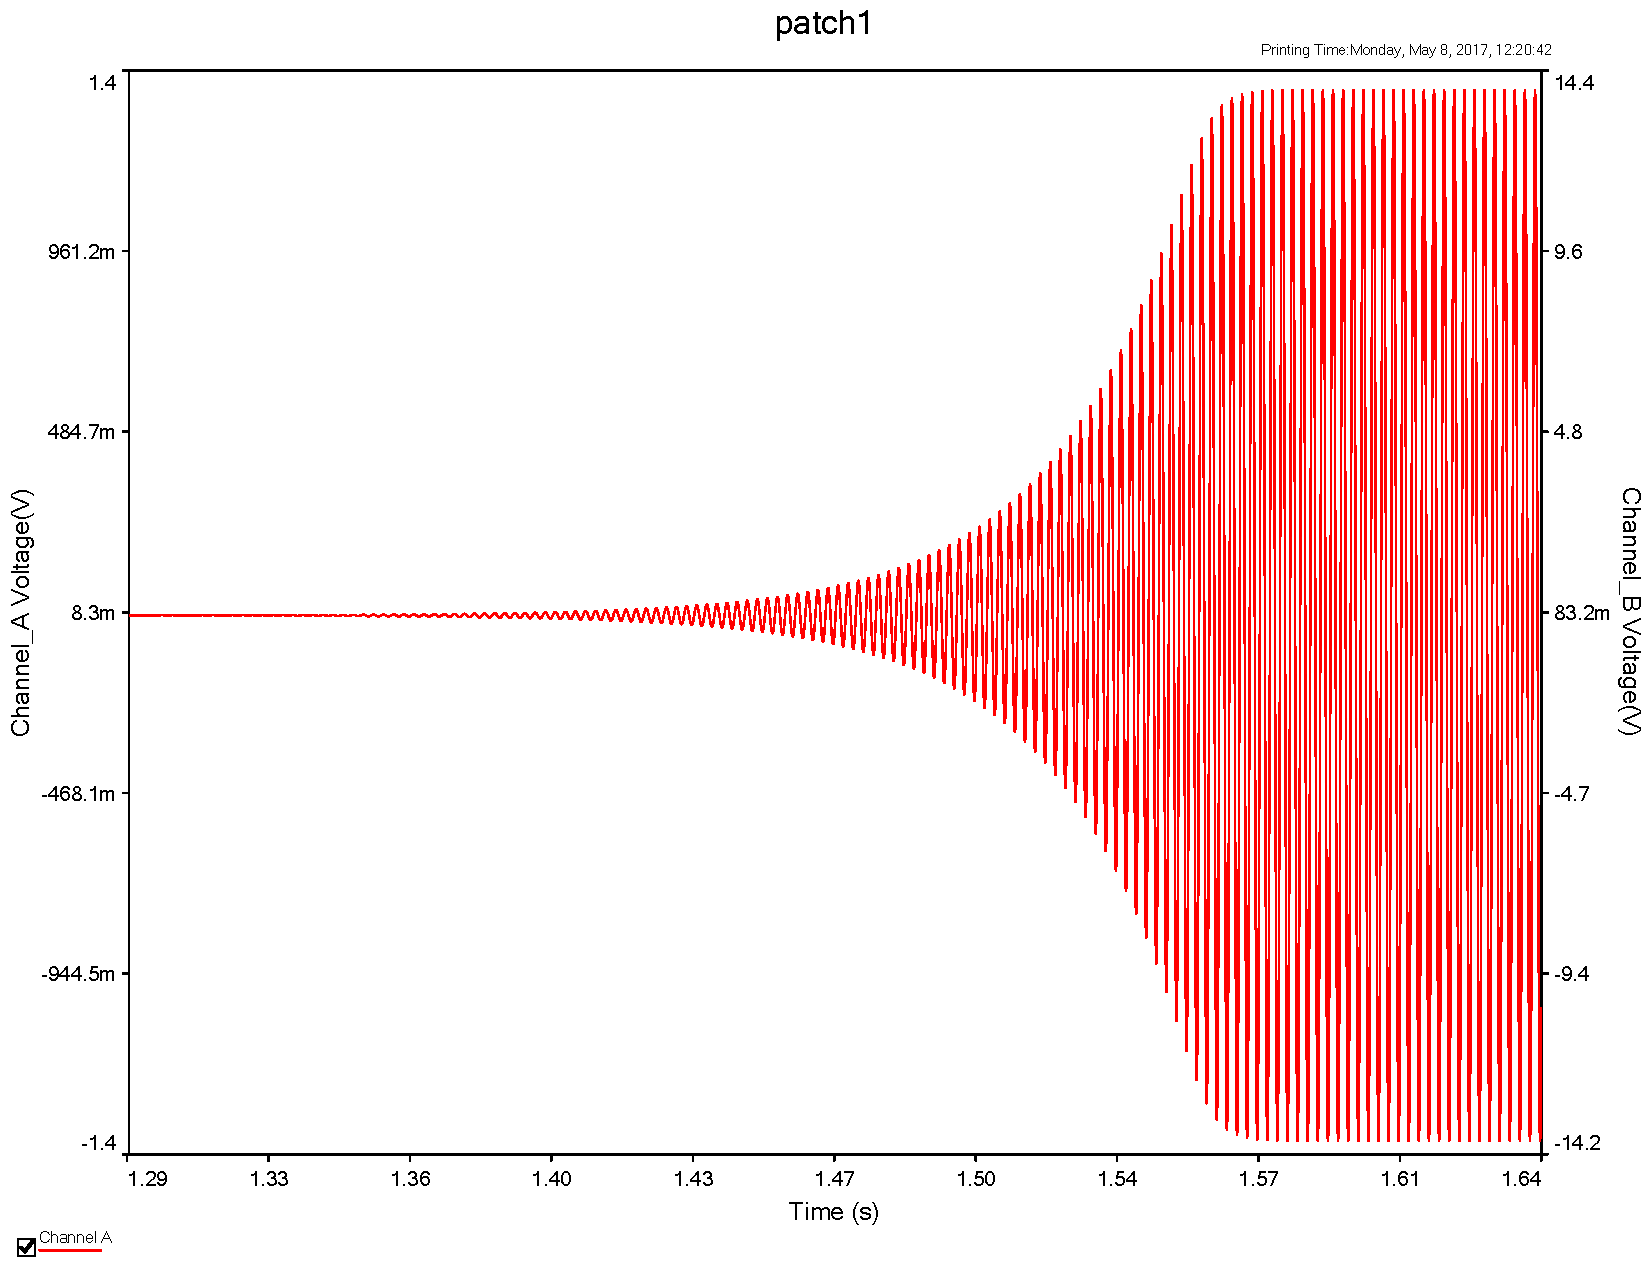
\includegraphics [width=\textwidth]{startac.pdf}
\caption{刚刚起振输出波形}
\label{ACstart}
\end {figure}
\begin{figure}
\centering
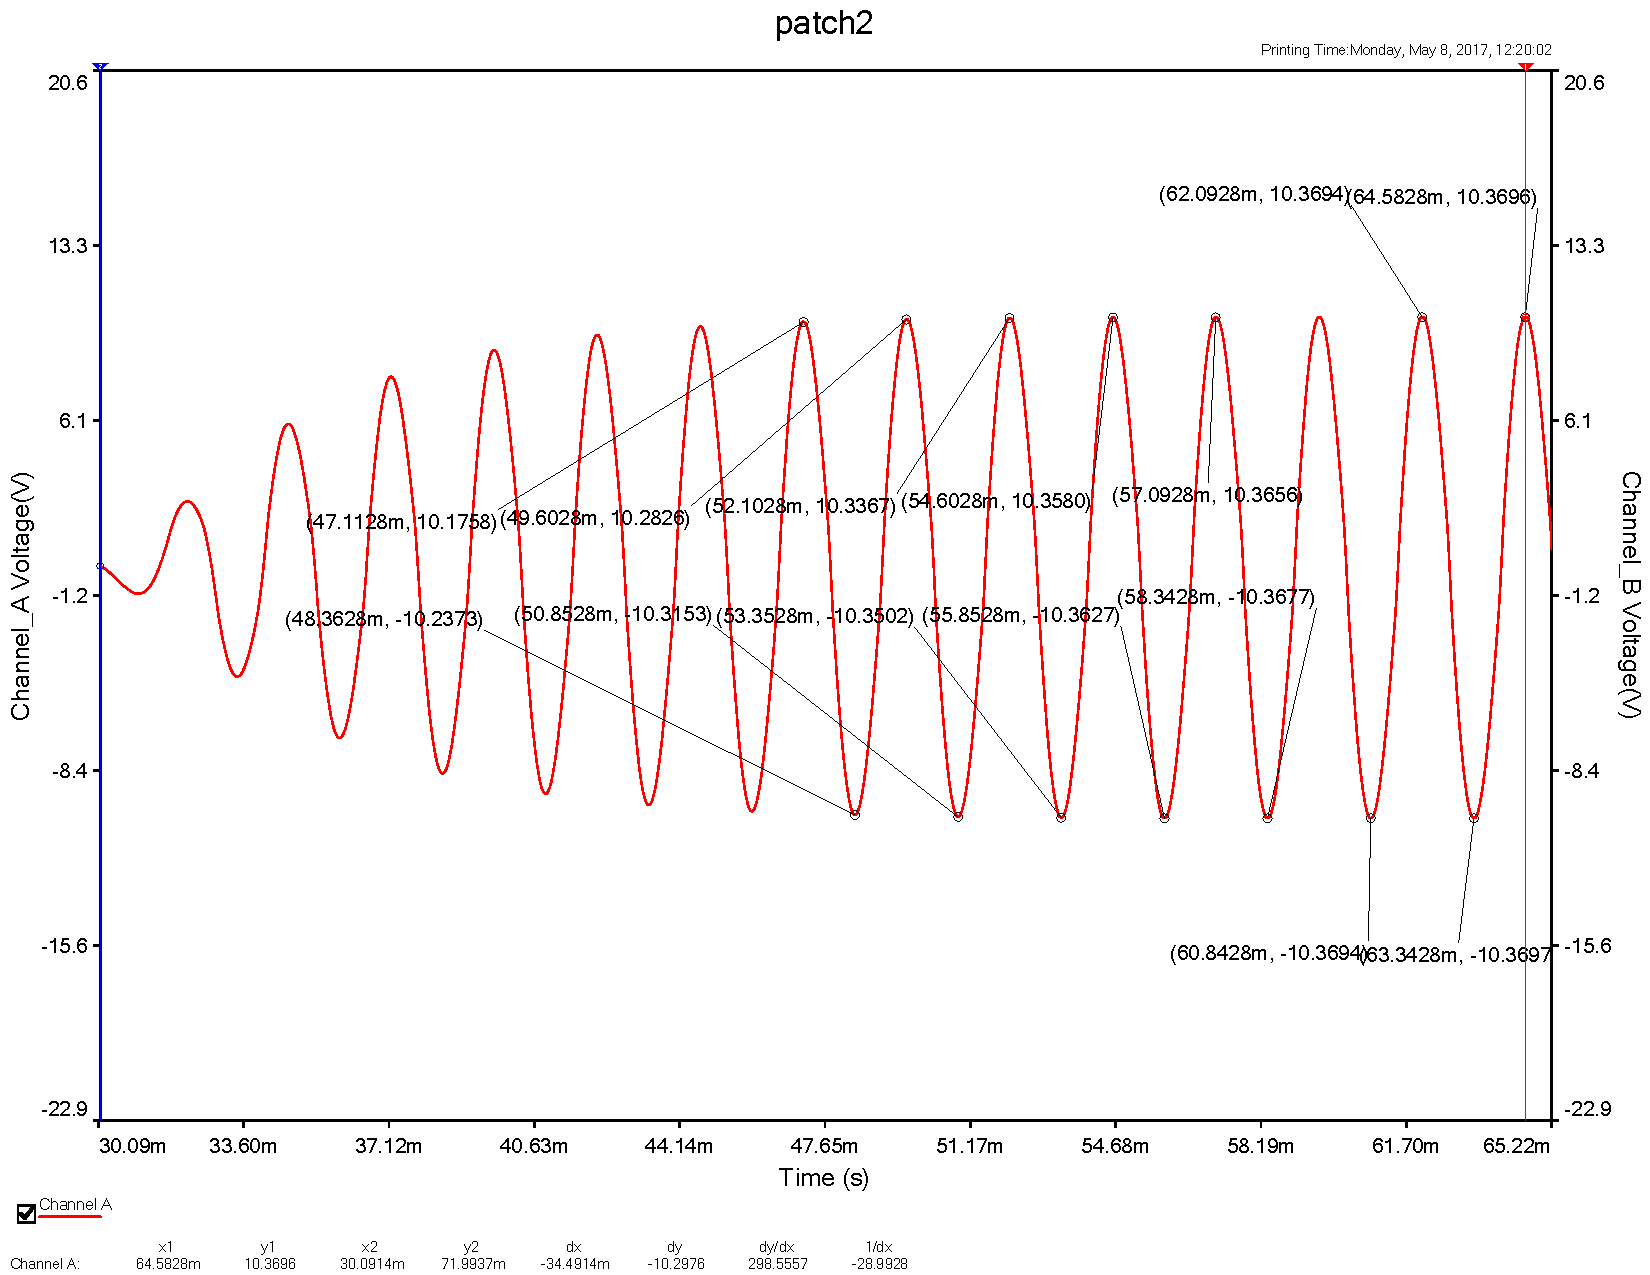
\includegraphics[width=\textwidth]{maxac.pdf}
\caption{输出最大不失真波形}
\label{ACmax}
\end{figure}
\clearpage
\subsubsection{其他情况的调试}
\begin{multicols}{2}
\begin{figure}[H]
\centering
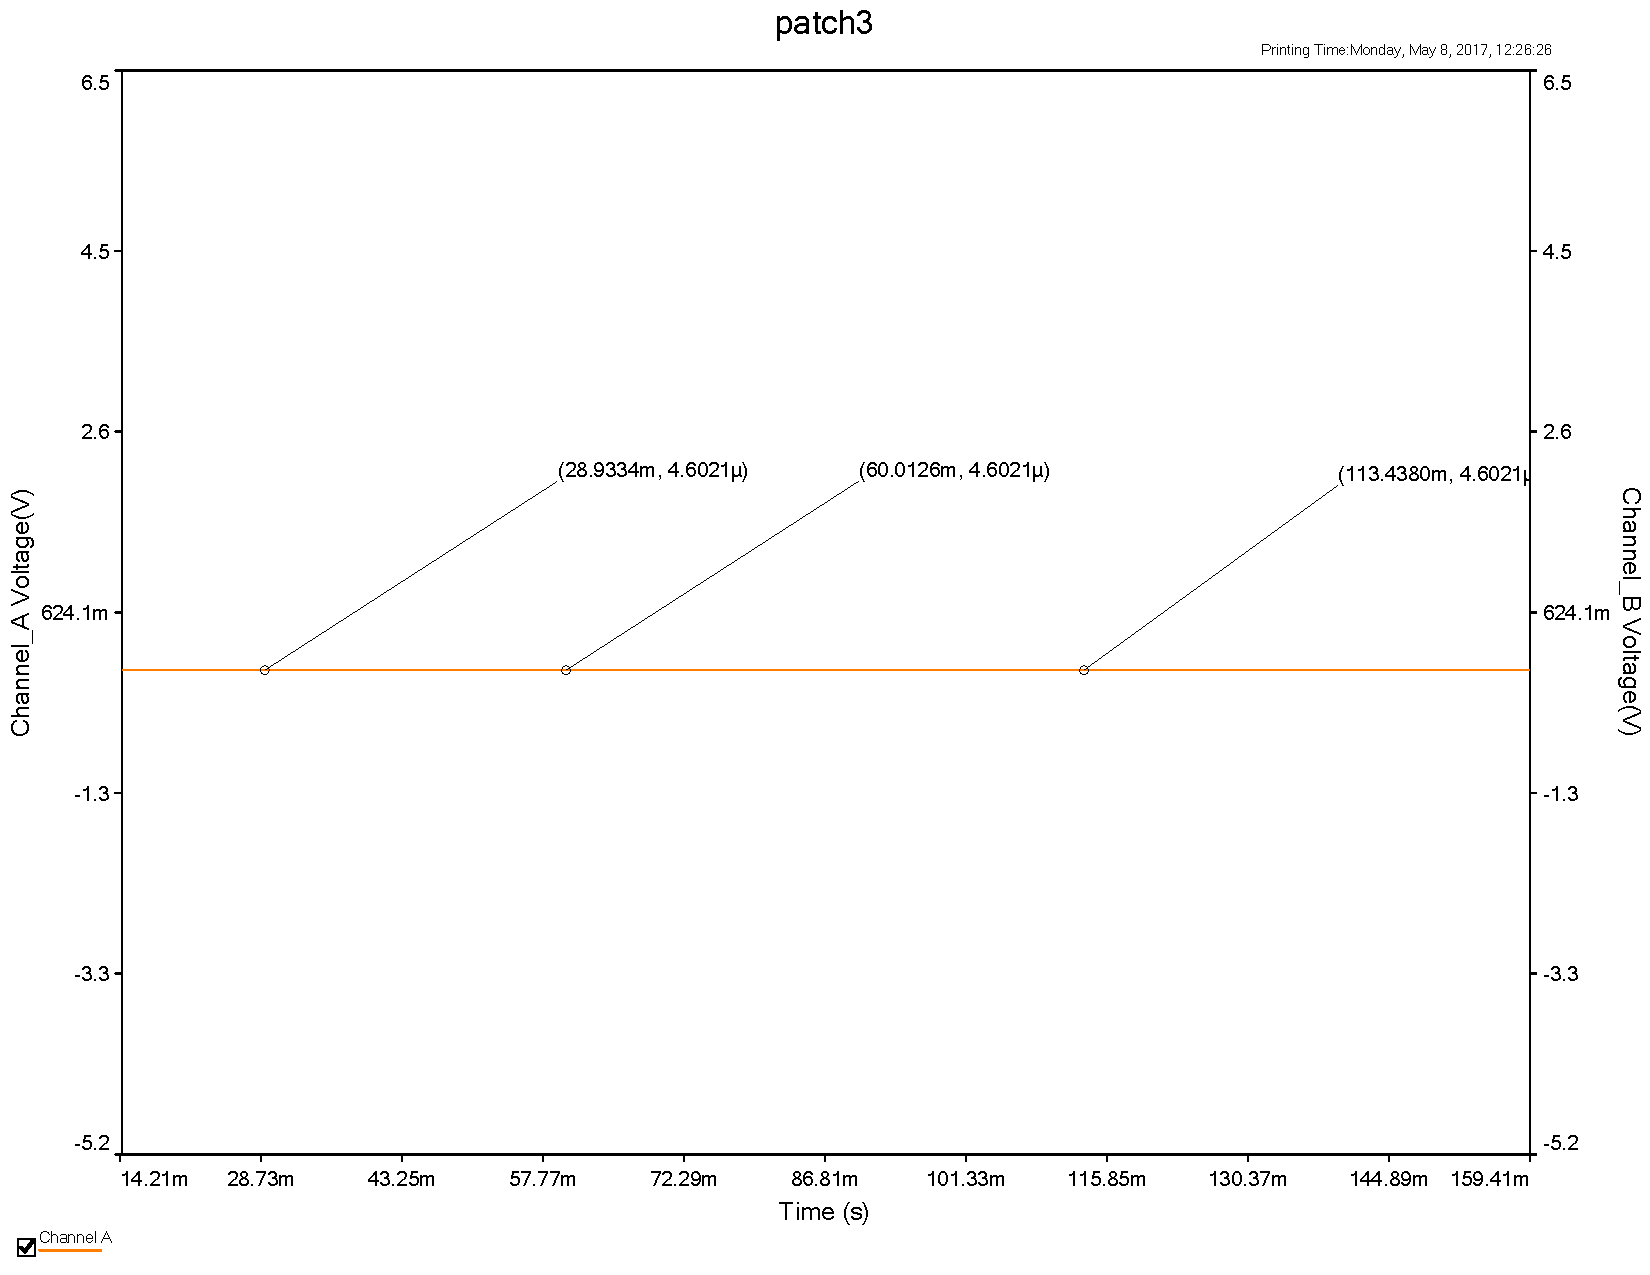
\includegraphics[width=\columnwidth]{0ac.pdf}
\caption{$R_w=20\%$时的输出波形}
\label{20}
\end{figure}
\begin{figure}[H]
\centering
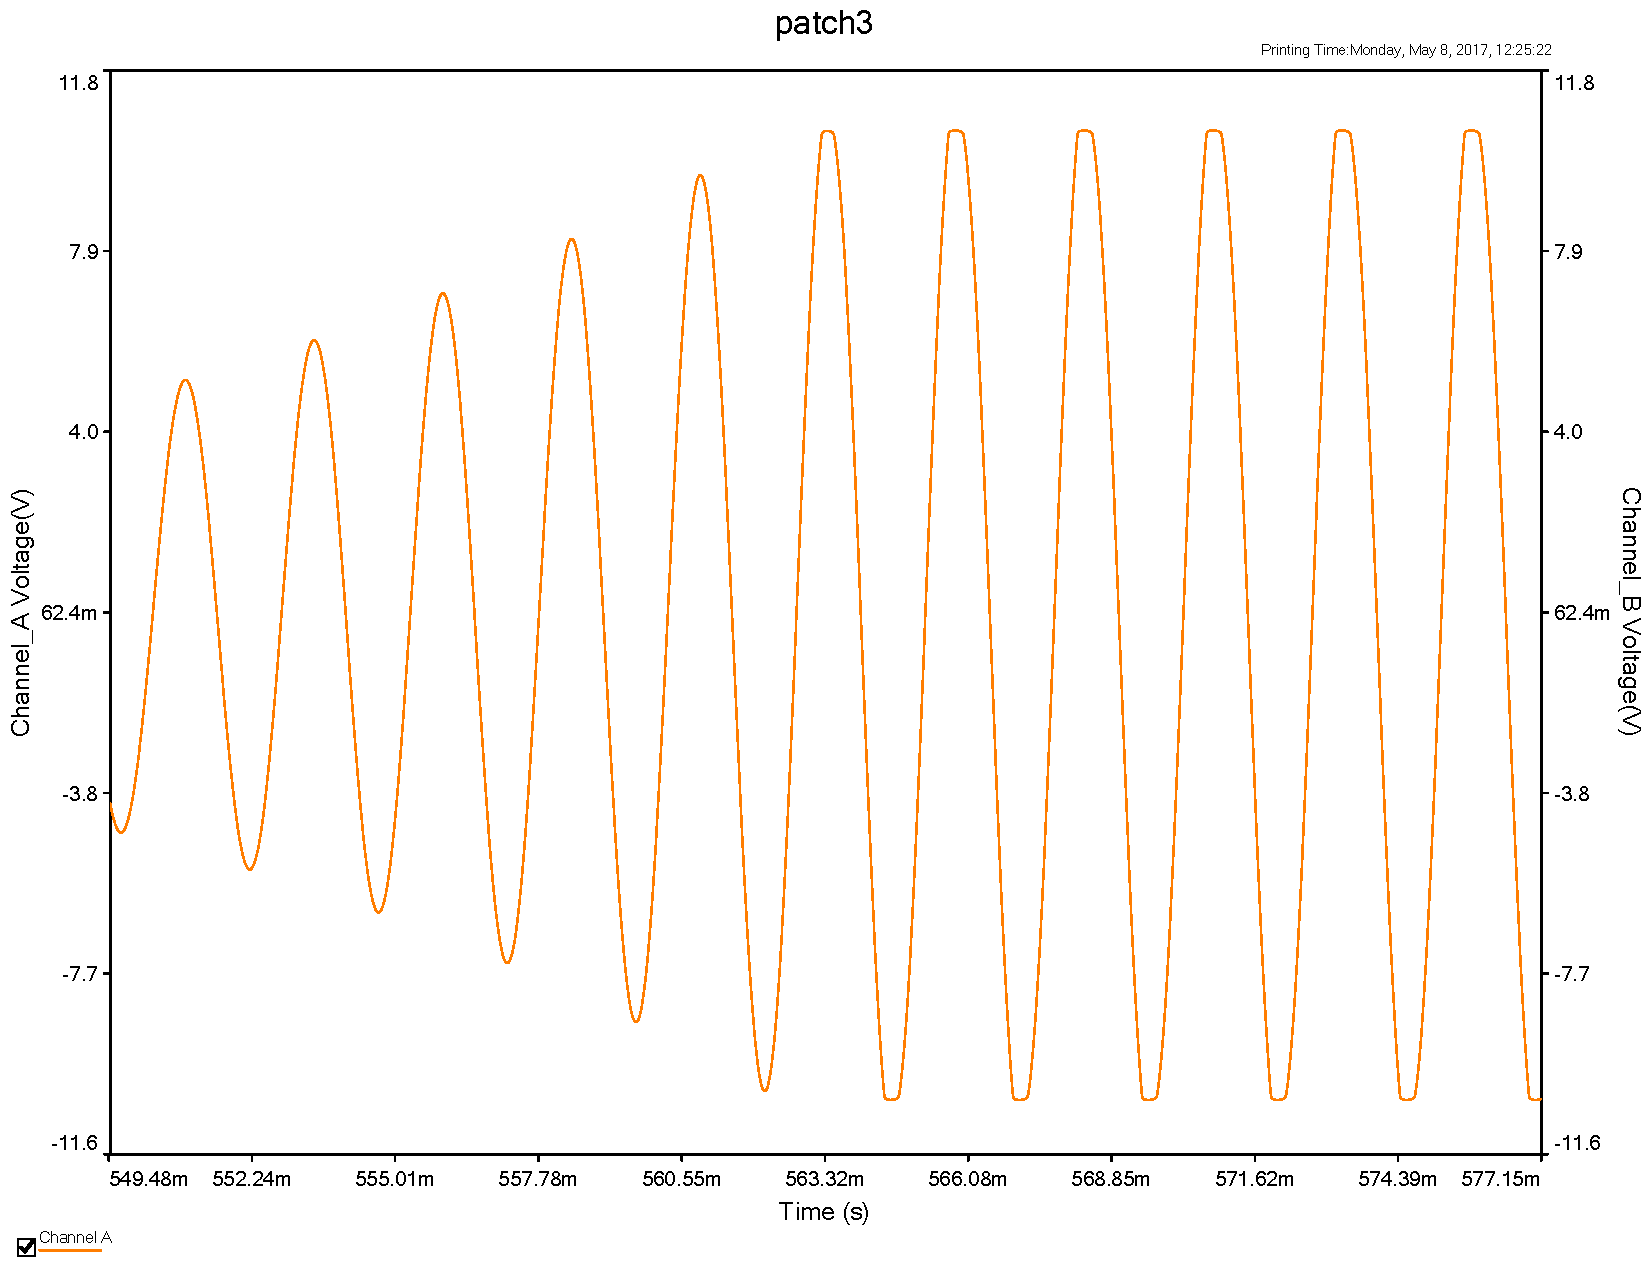
\includegraphics[width=\columnwidth]{21ac.pdf}
\caption{$R_w=21\%$时的输出波形}
\label{21}
\end{figure}
\begin{figure}[H]
\centering
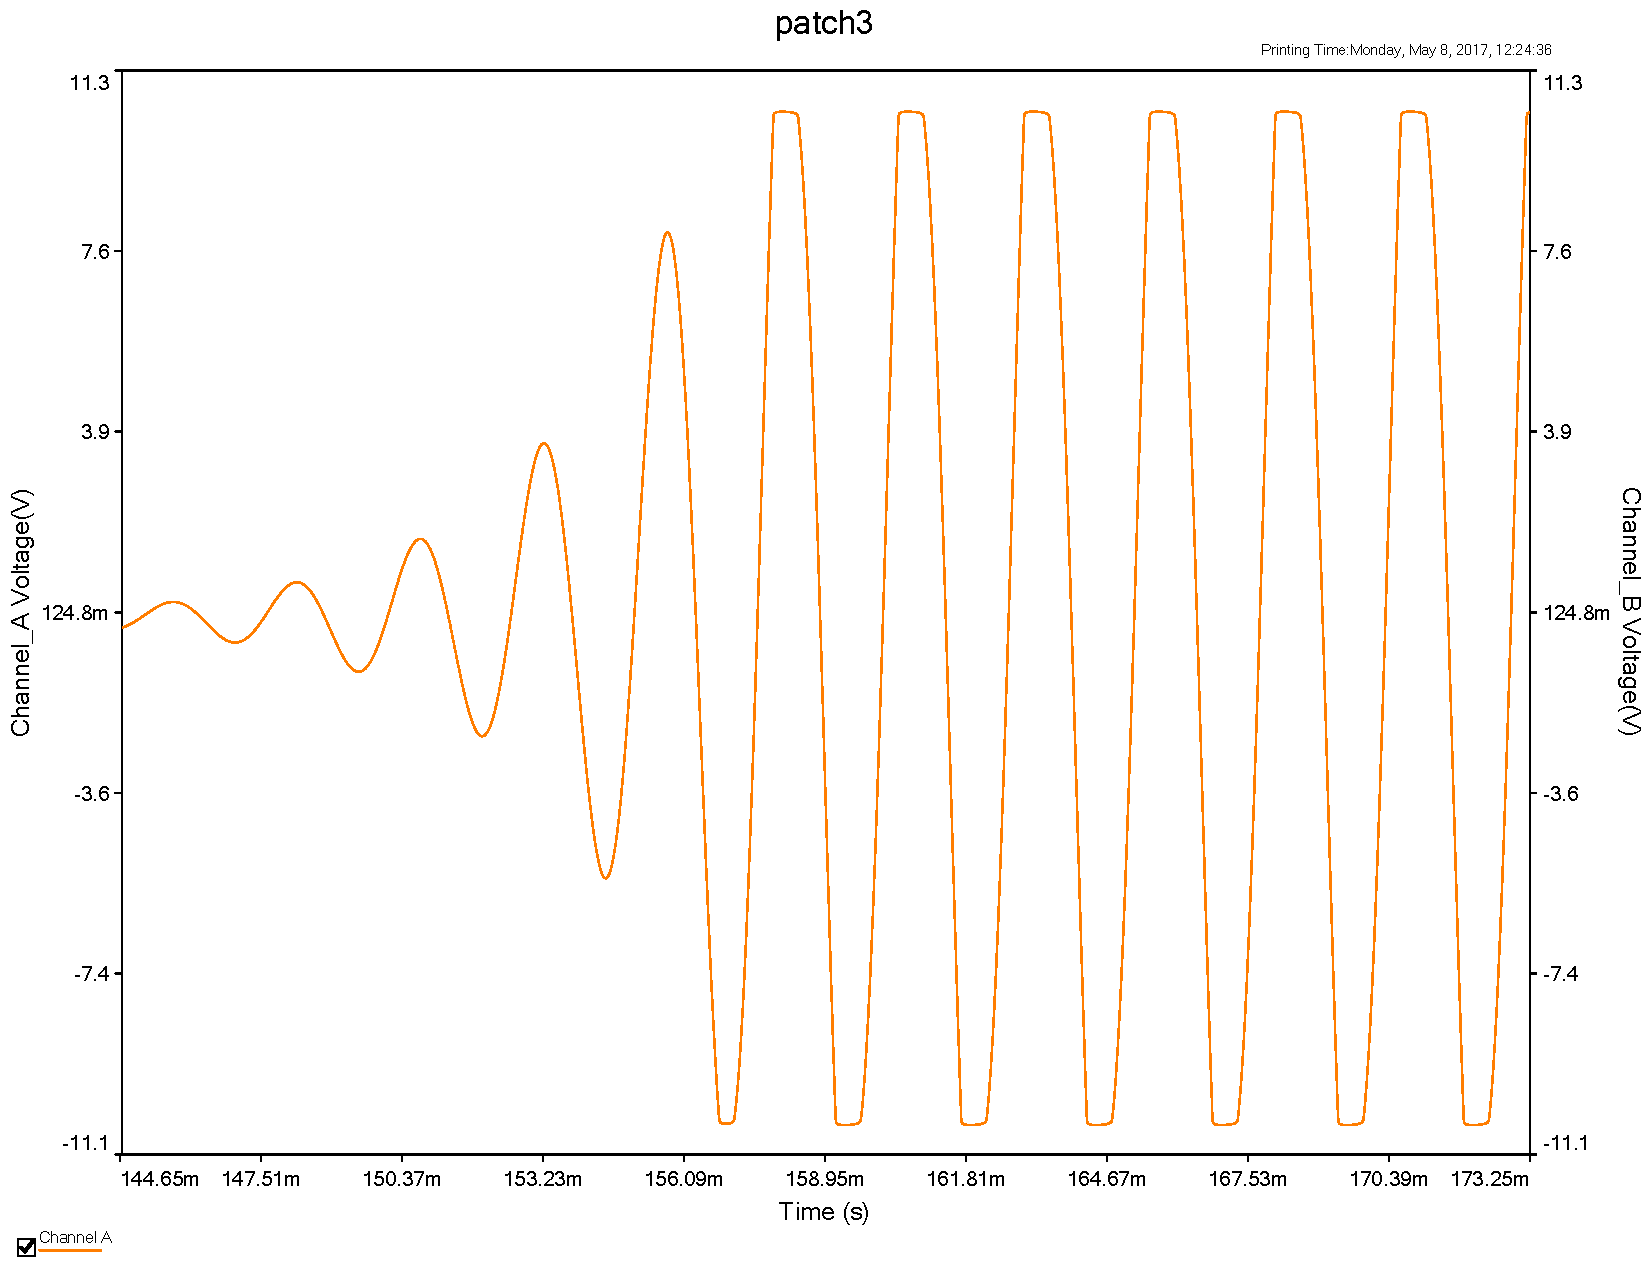
\includegraphics[width=\columnwidth]{25ac.pdf}
\caption{$R_w=25\%$时的输出波形}
\label{25}
\end{figure}
\begin{figure}[H]
\centering
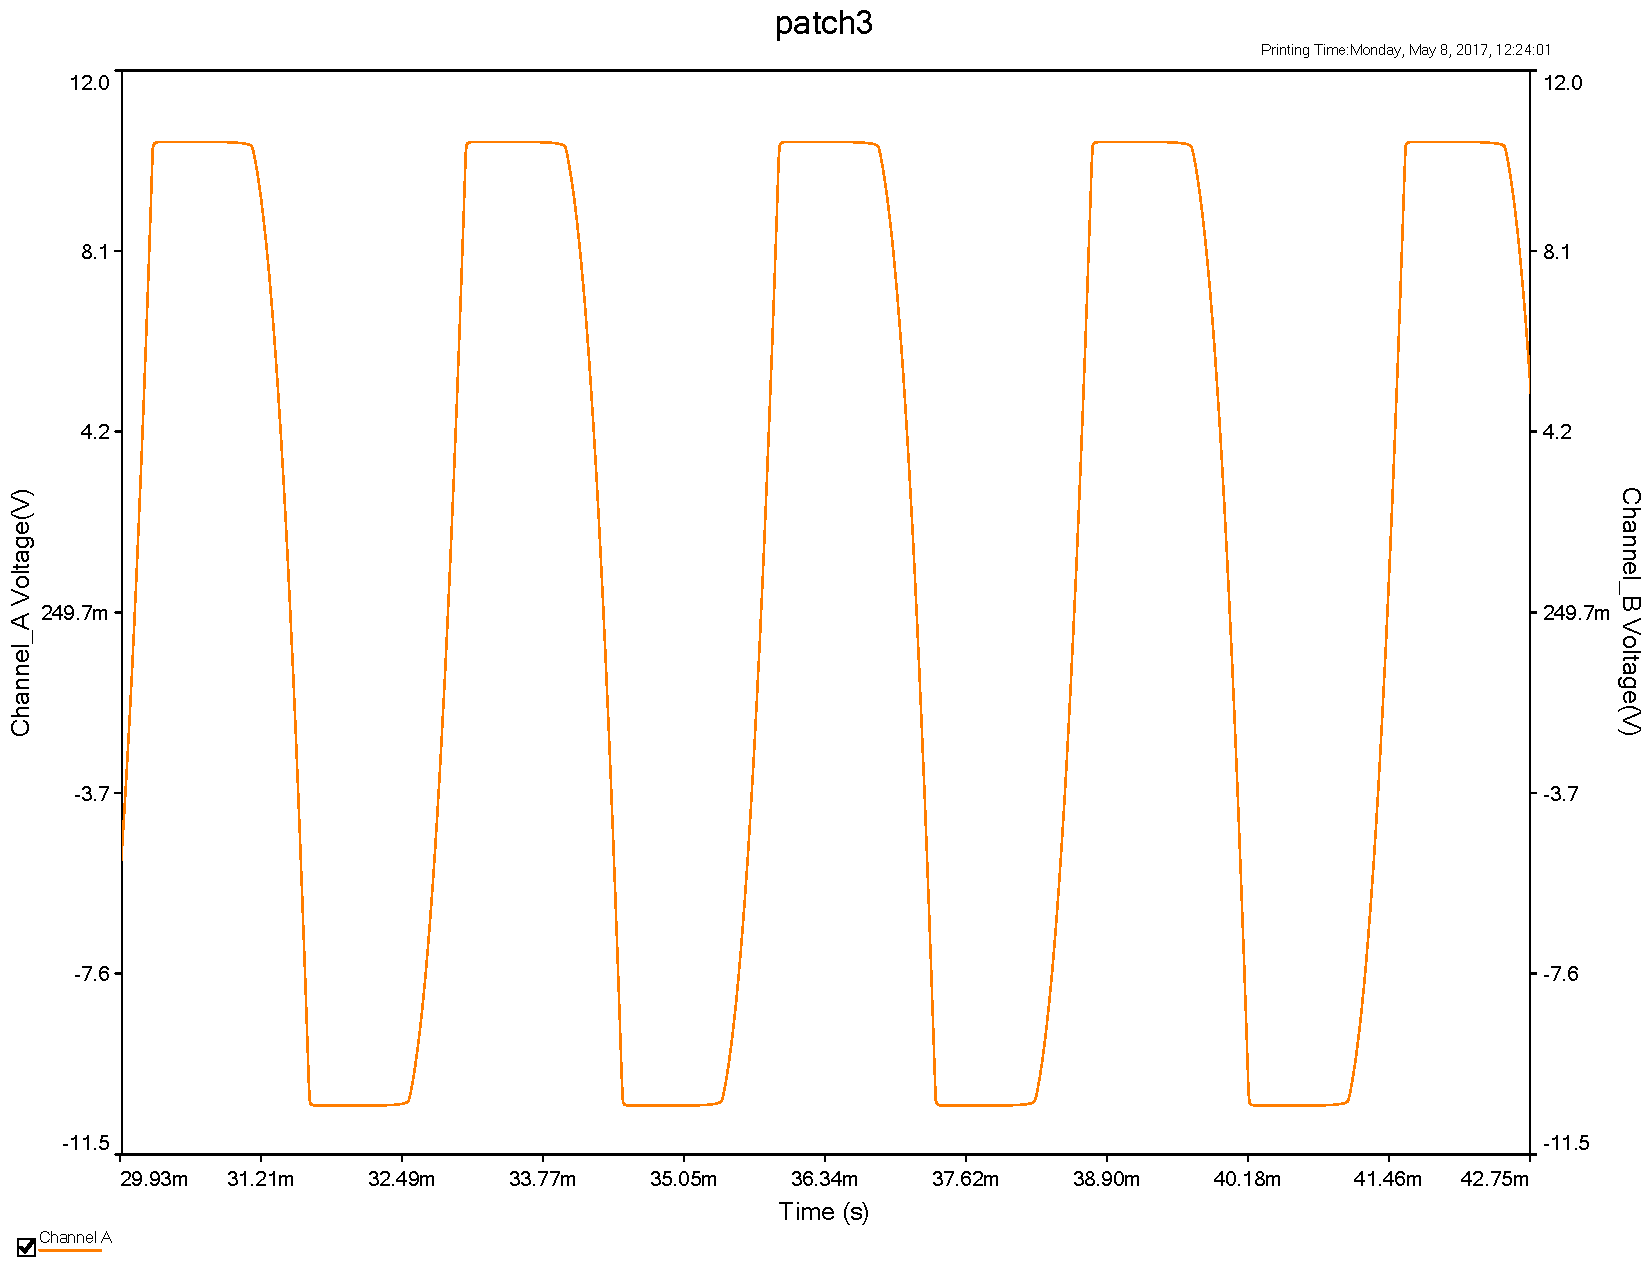
\includegraphics[width=\columnwidth]{40ac.pdf}
\caption{$R_w=40\%$时的输出波形}
\label{40}
\end{figure}
\begin{figure}[H]
\centering
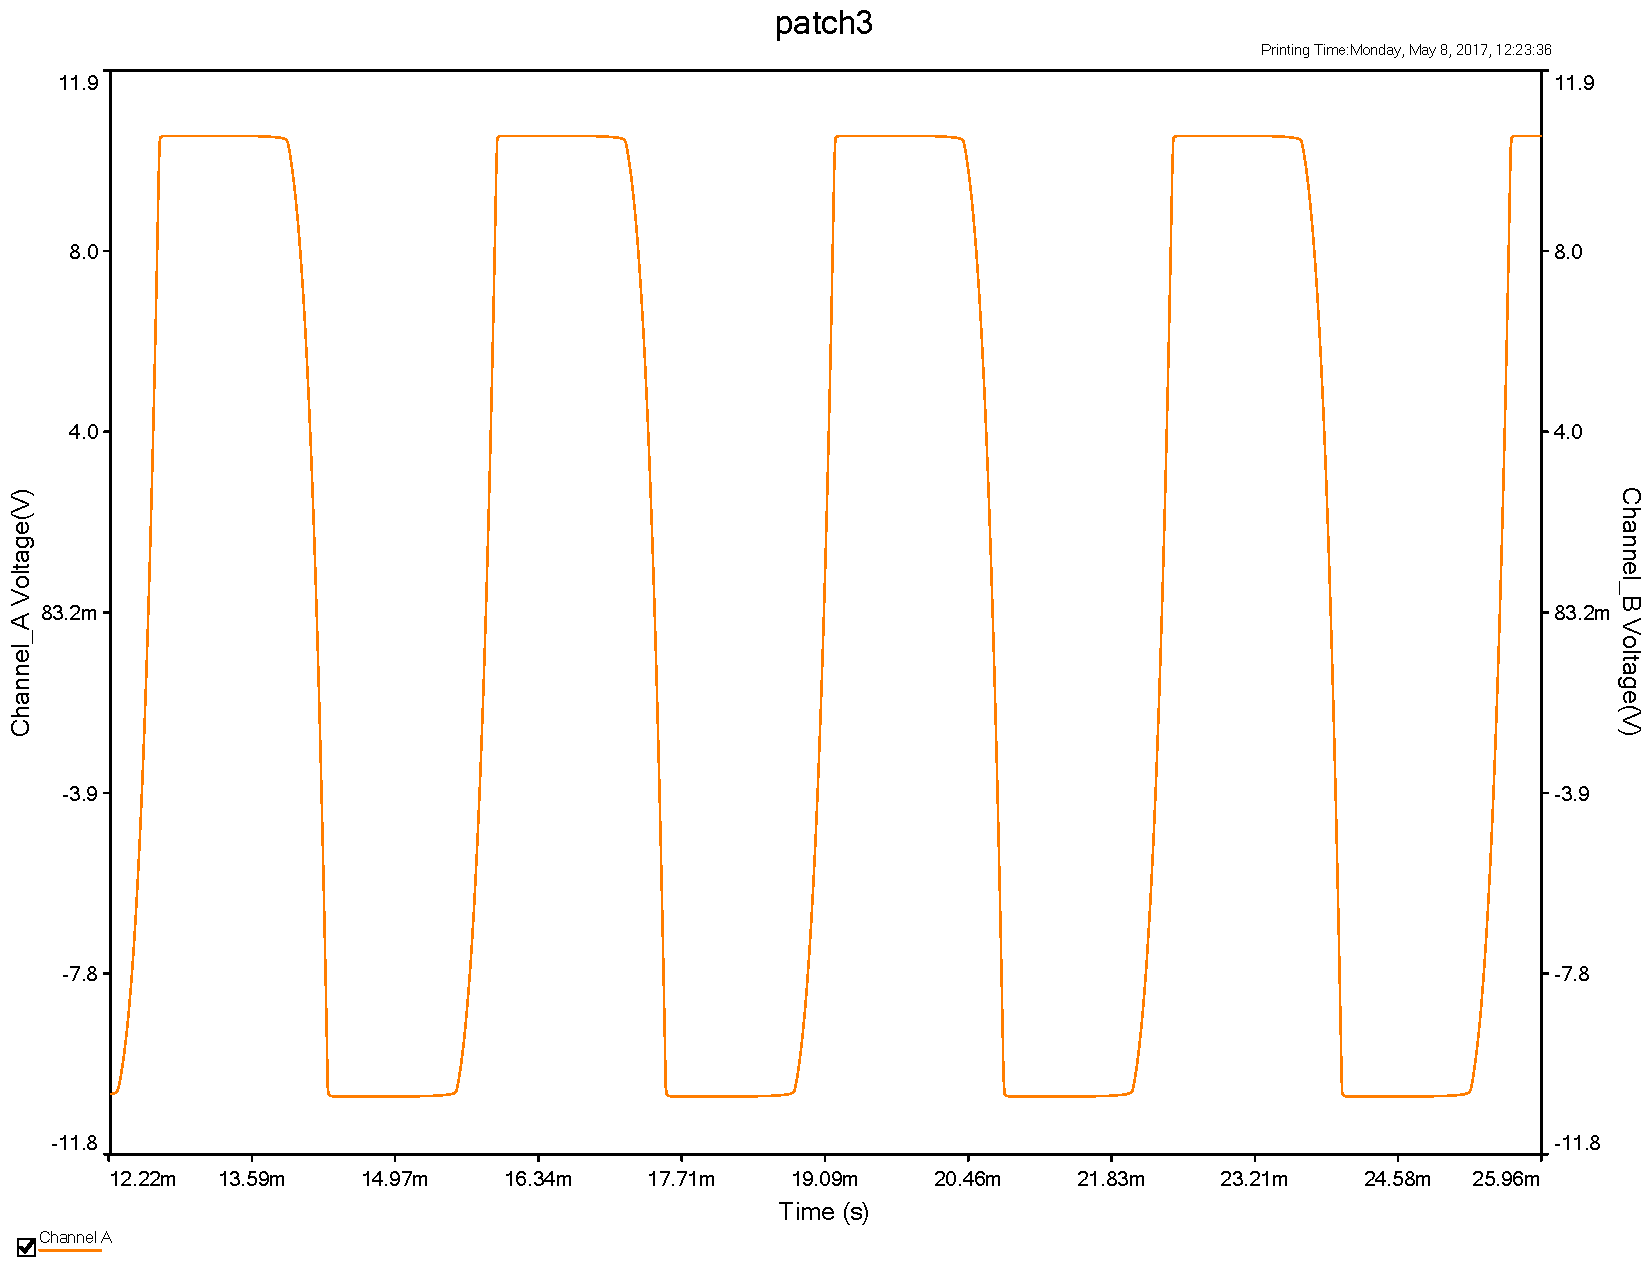
\includegraphics[width=\columnwidth]{60ac.pdf}
\caption{$R_w=60\%$时的输出波形}
\label{60}
\end{figure}
\begin{figure}[H]
\centering
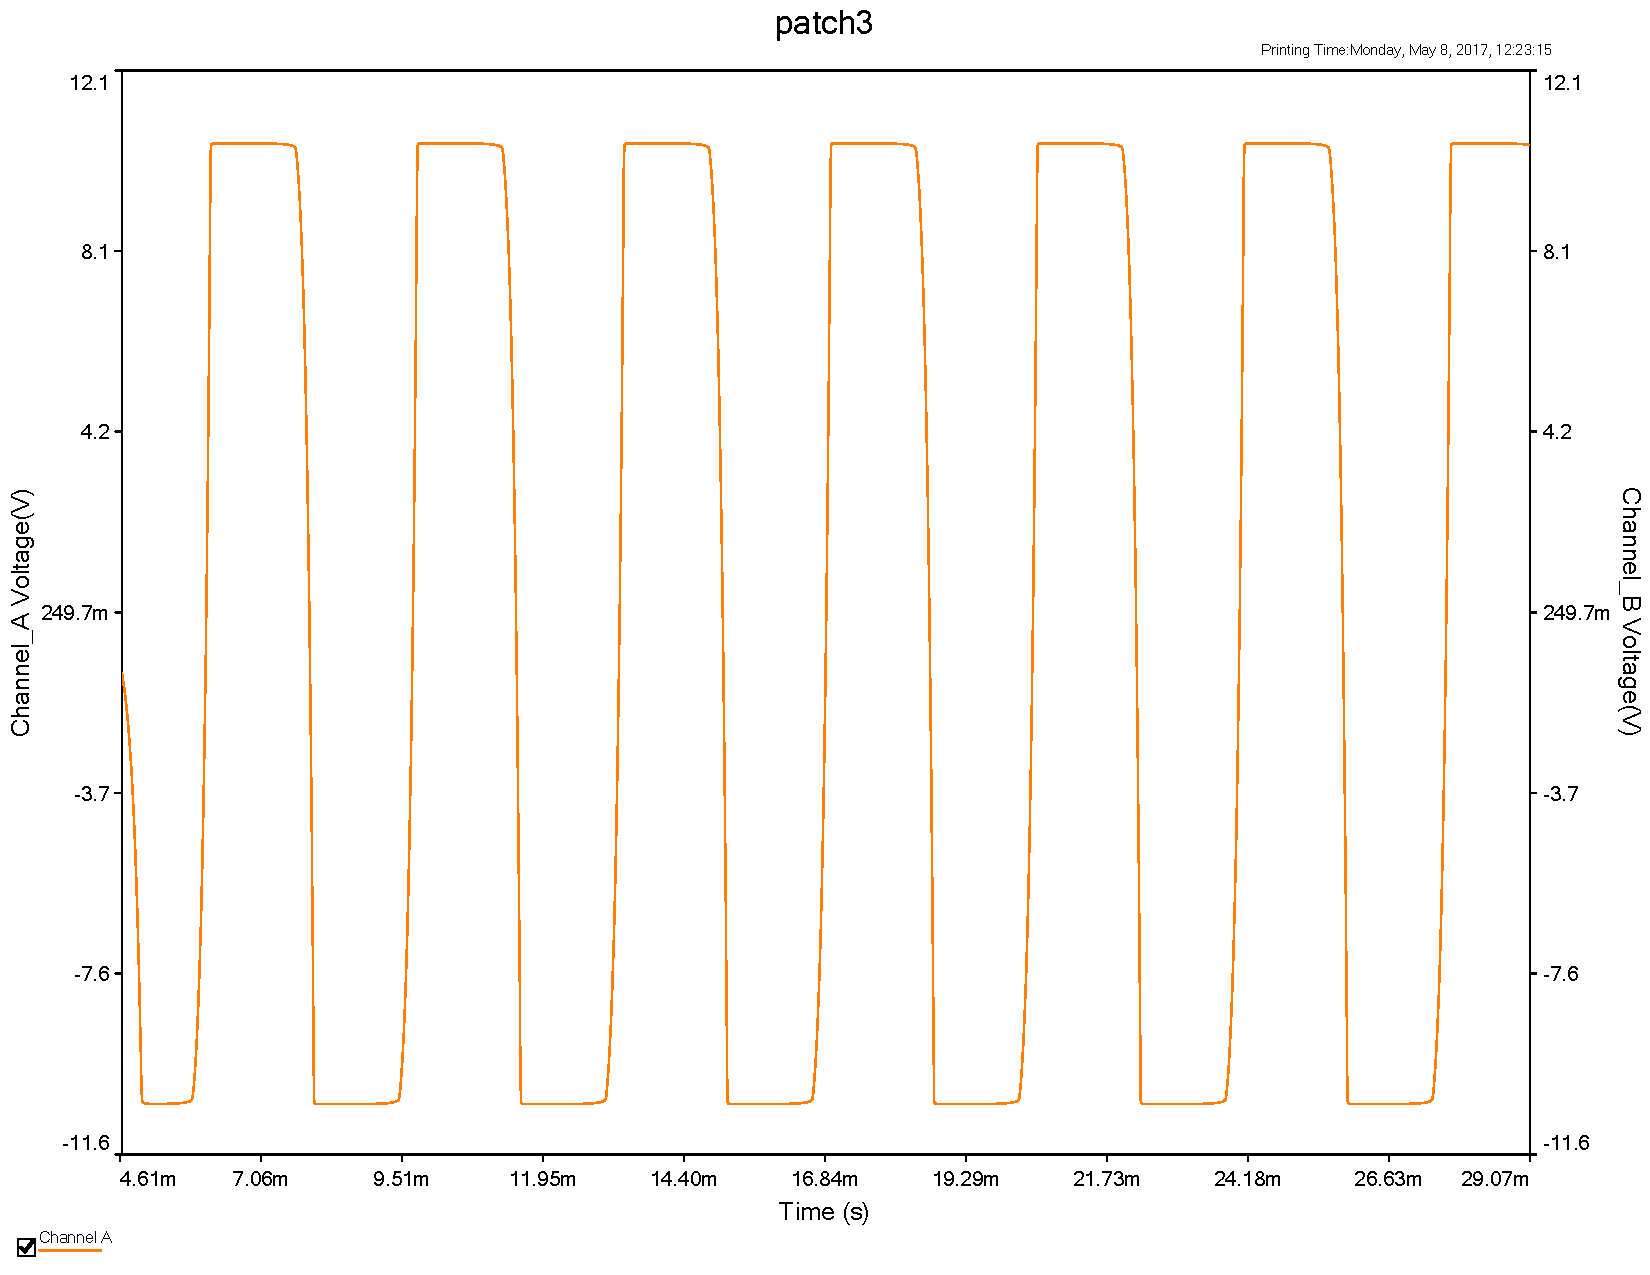
\includegraphics[width=\columnwidth]{80ac.pdf}
\caption{$R_w=80\%$时的输出波形}
\label{80}
\end{figure}
\begin{figure}[H]
\centering
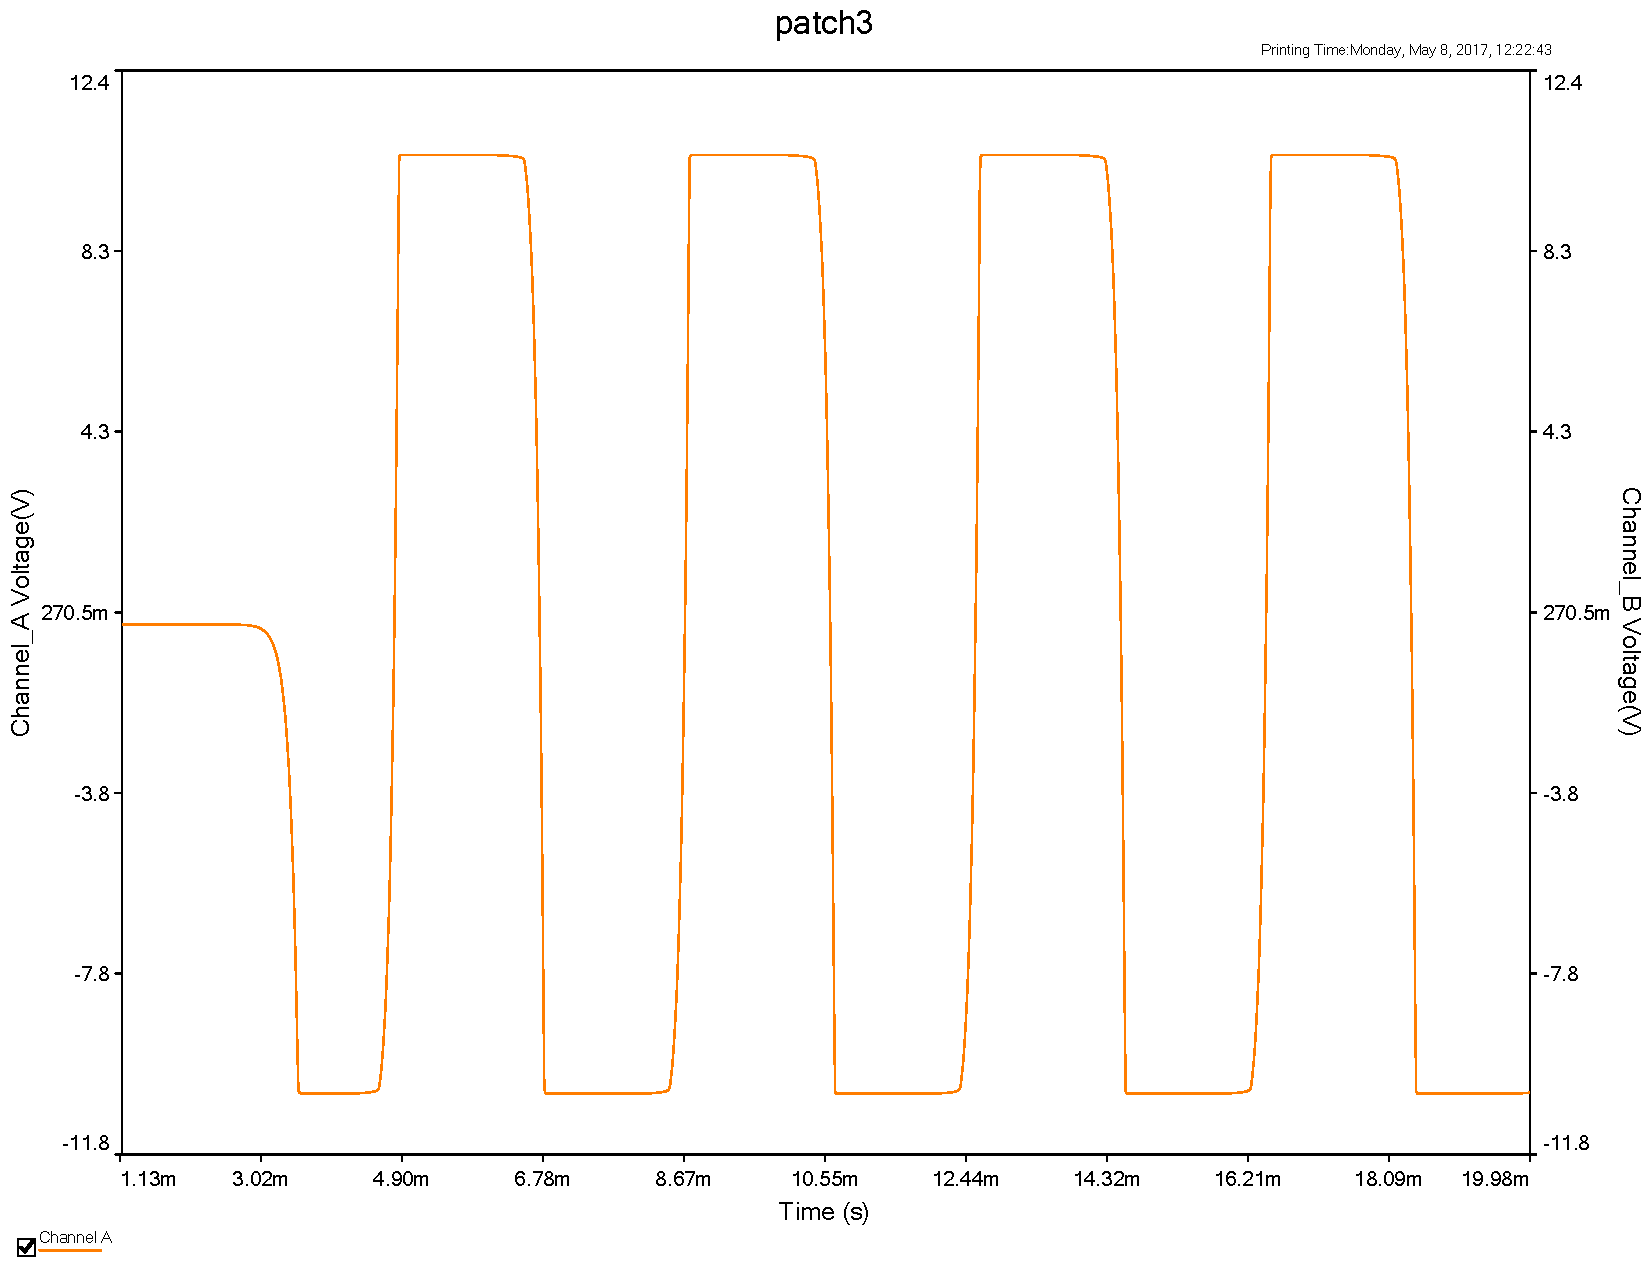
\includegraphics[width=\columnwidth]{100ac.pdf}
\caption{$R_w=100\%$时的输出波形}
\label{100}
\end{figure}
\begin{figure}[H]
\centering
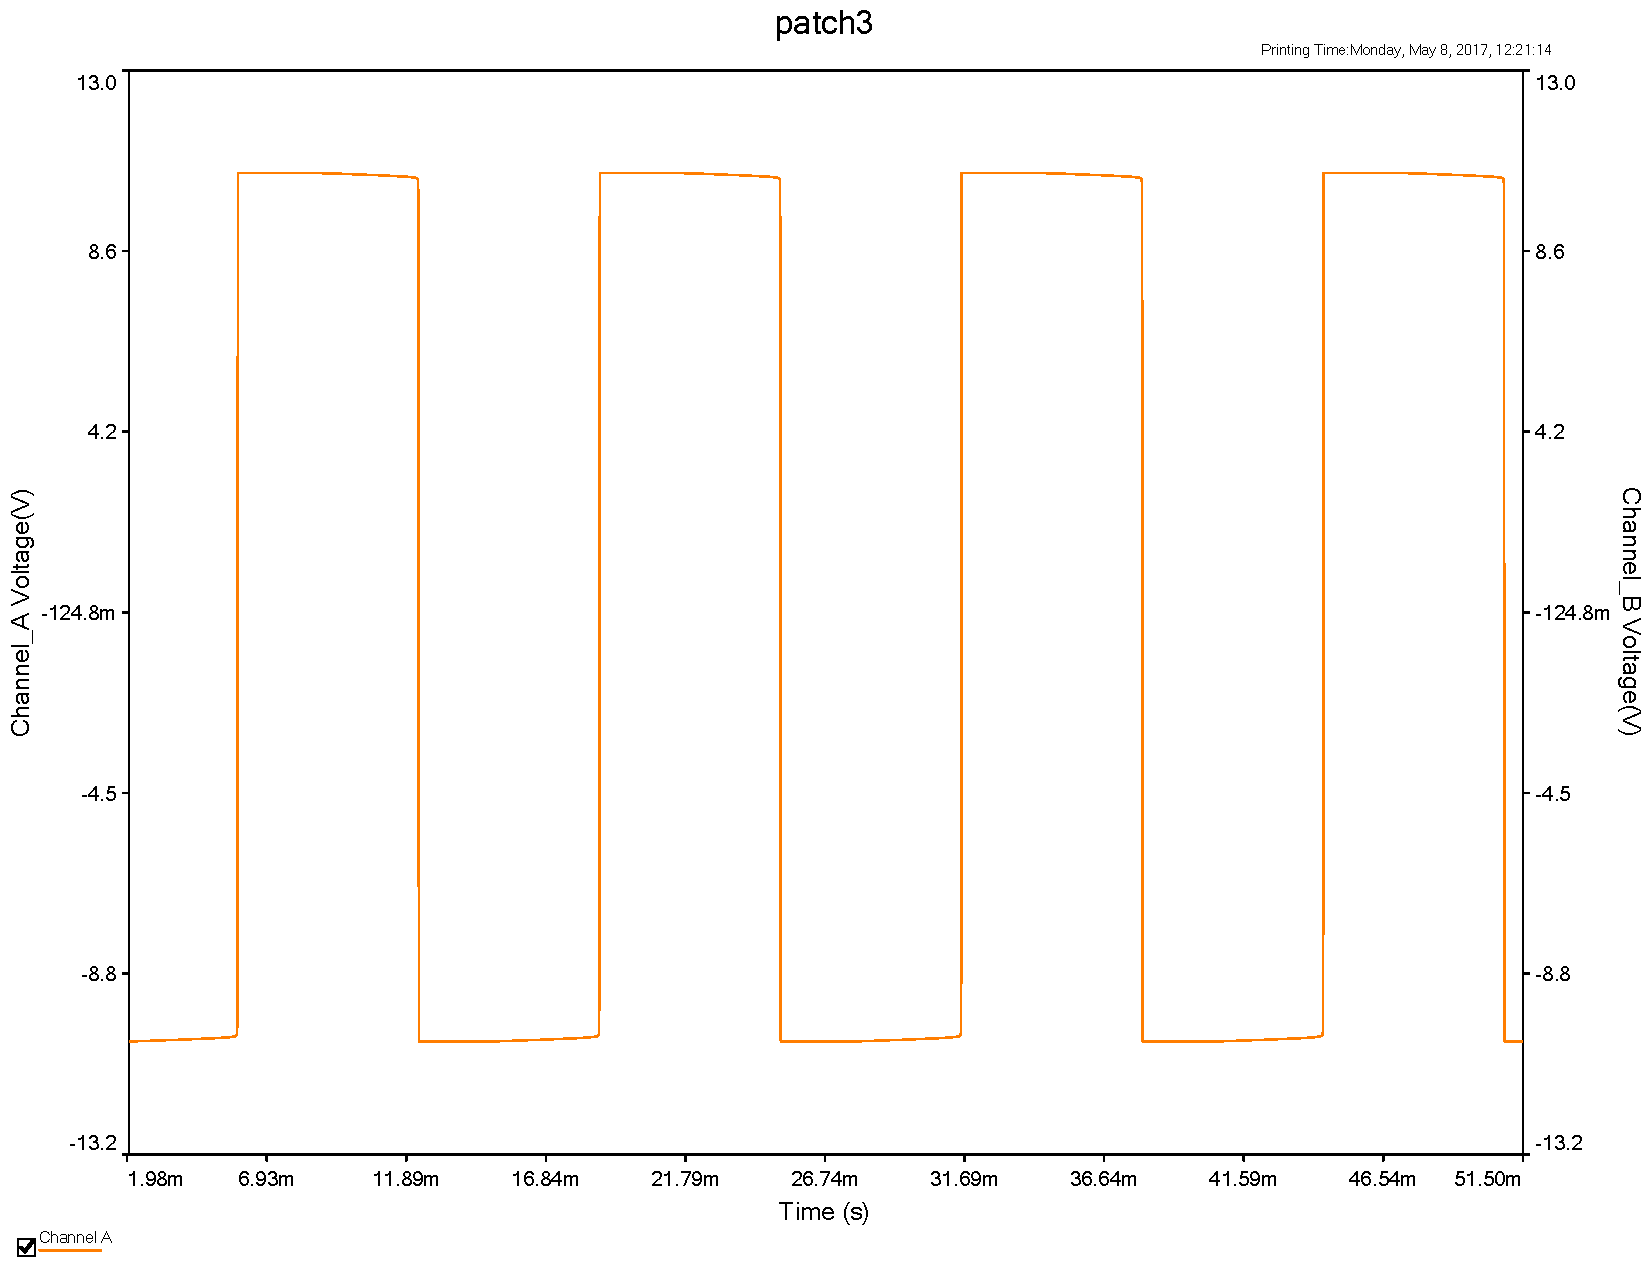
\includegraphics[width=\columnwidth]{offac.pdf}
\caption{$R_w$完全断开时的输出波形}
\label{infi}
\end{figure}
\end{multicols}
\subsection{方波——三角波发生电路}
\subsubsection{理论分析}
\label{sec:}
\begin{multicols}{2}
如图\ref{BICirc}是方波——三角波发生电路的电路图

首先对电路进行理论估计,为了和实验值保持一致,改用了和实验室提供的稳压管相同导通压降$U_Z=5.1\mathrm{V}$的稳压管1N4733A,得到左侧同相输入滞环特性的阈值电压方程
$$\frac{R_1}{R_1+R_2}U_T\pm\frac{R_2}{R_1+R_2}U_Z=0$$
得到
$$U_T=\pm\frac{R_2}{R_1}U_Z=2.55\mathrm{V}$$
右侧电路为积分运算电路,输出电压的表达式为
$$U_0=\int U_Z\mathrm{d}t$$半个周期内积分从$-U_T$抵达$+U_T$,因此可以得到$$2U_T=\frac{T}{2}\frac{U_Z}{R_4C}$$,结合前几式可以得到$$T=\frac{4R_2R_4C}{R_1}=0.4\mathrm{mS}$$
\begin {figure}[H]
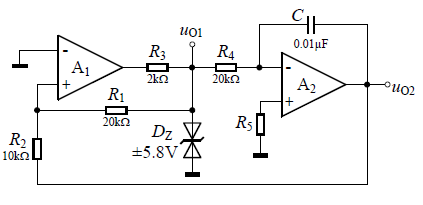
\includegraphics [width=\columnwidth]{bi.png}
\caption{方波——三角波发生电路}
\label{BICirc}
\end {figure}
\end{multicols}
\subsubsection{波形仿真}
\begin{figure}
\centering
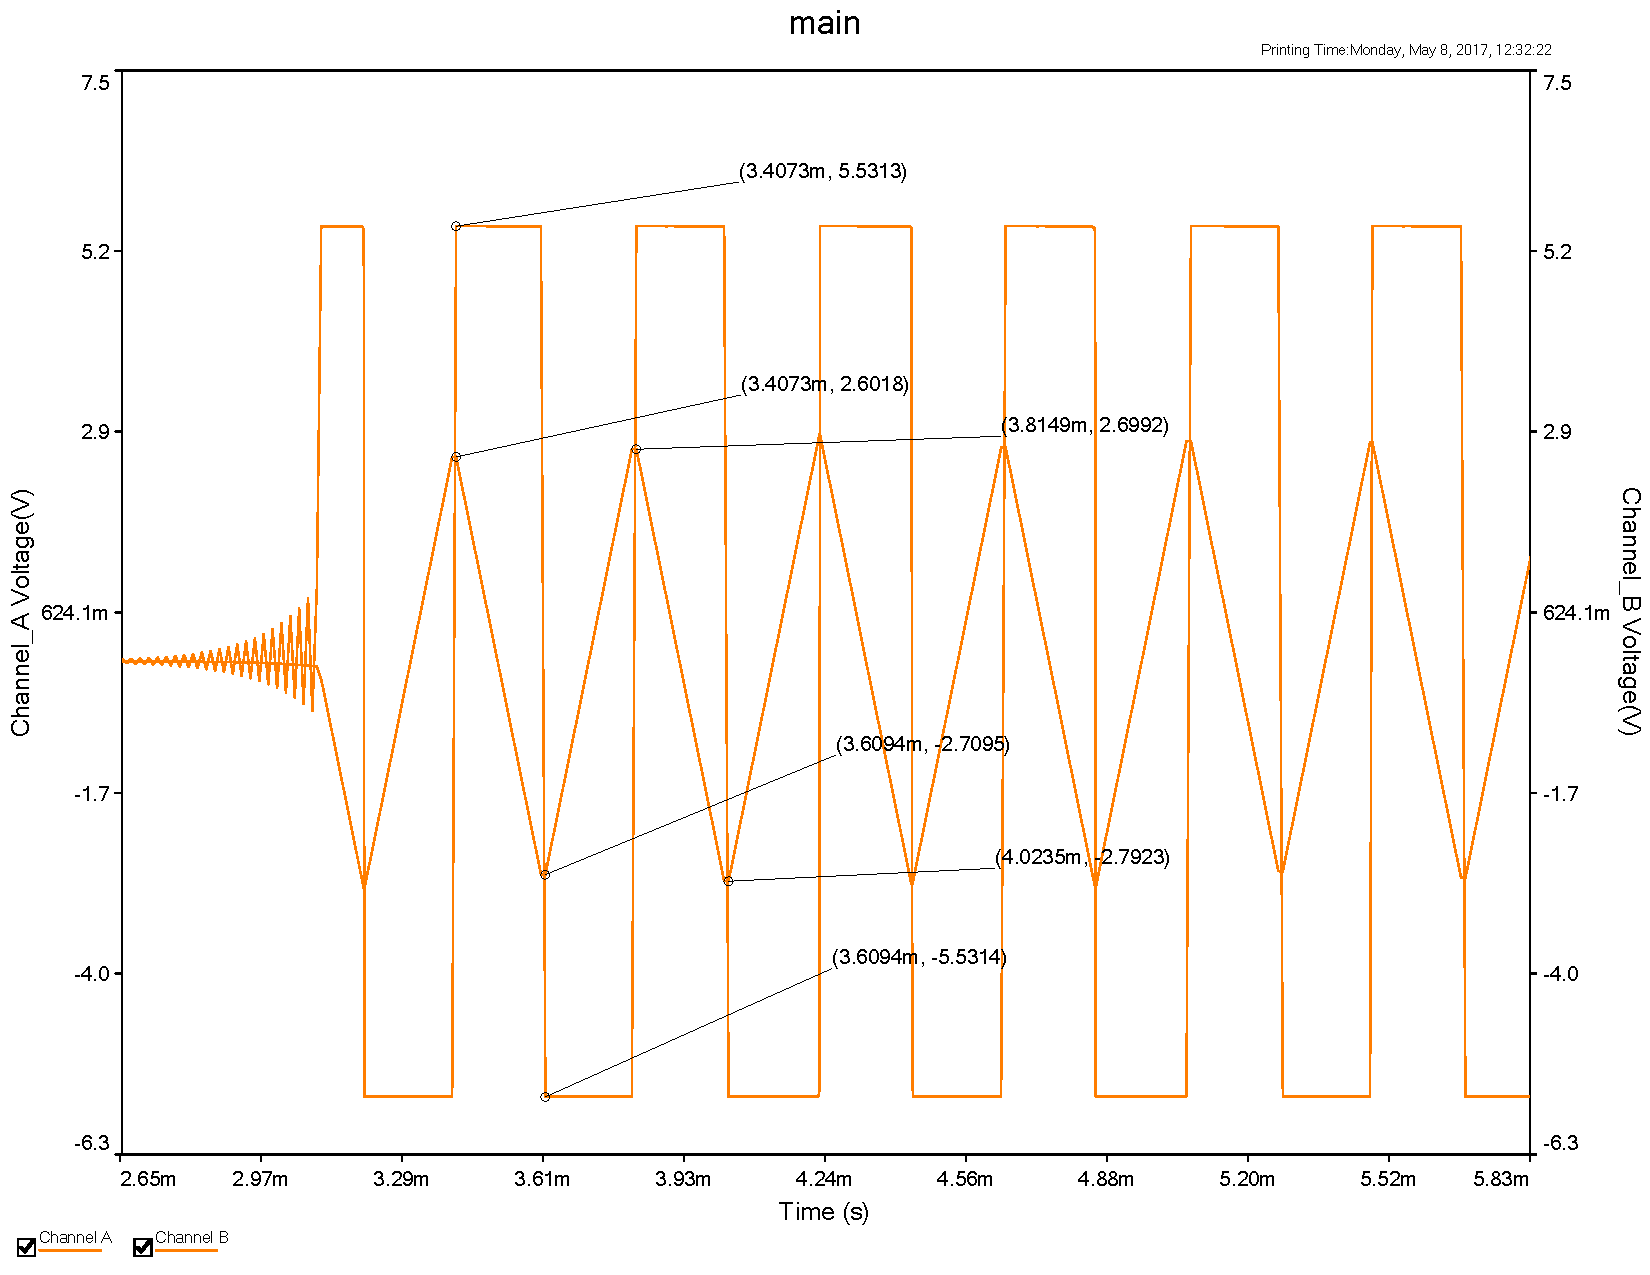
\includegraphics[width=\textwidth]{bi.pdf}
\caption{方波——三角波发生电路输出波形}
\label{BI}
\end{figure}
\subsection{滞环特性电路的测试}
\subsubsection{理论分析}
如图\ref{schiCrit}是滞环特性电路电路图,有关$U_T$的推导的问题可以参阅\ref{sec:}节的说明,这里就不加重复了。
\begin {figure}
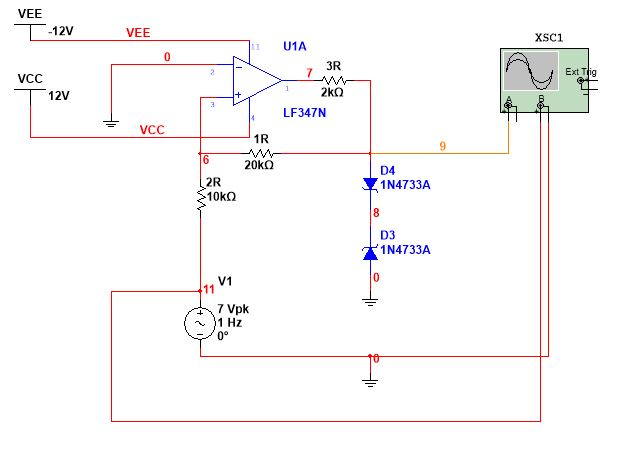
\includegraphics [width=\textwidth]{sch.jpg}
\caption{滞环特性电路}
\label{schiCrit}
\end {figure}
\subsubsection{输出波形仿真}
\begin{figure}
\centering
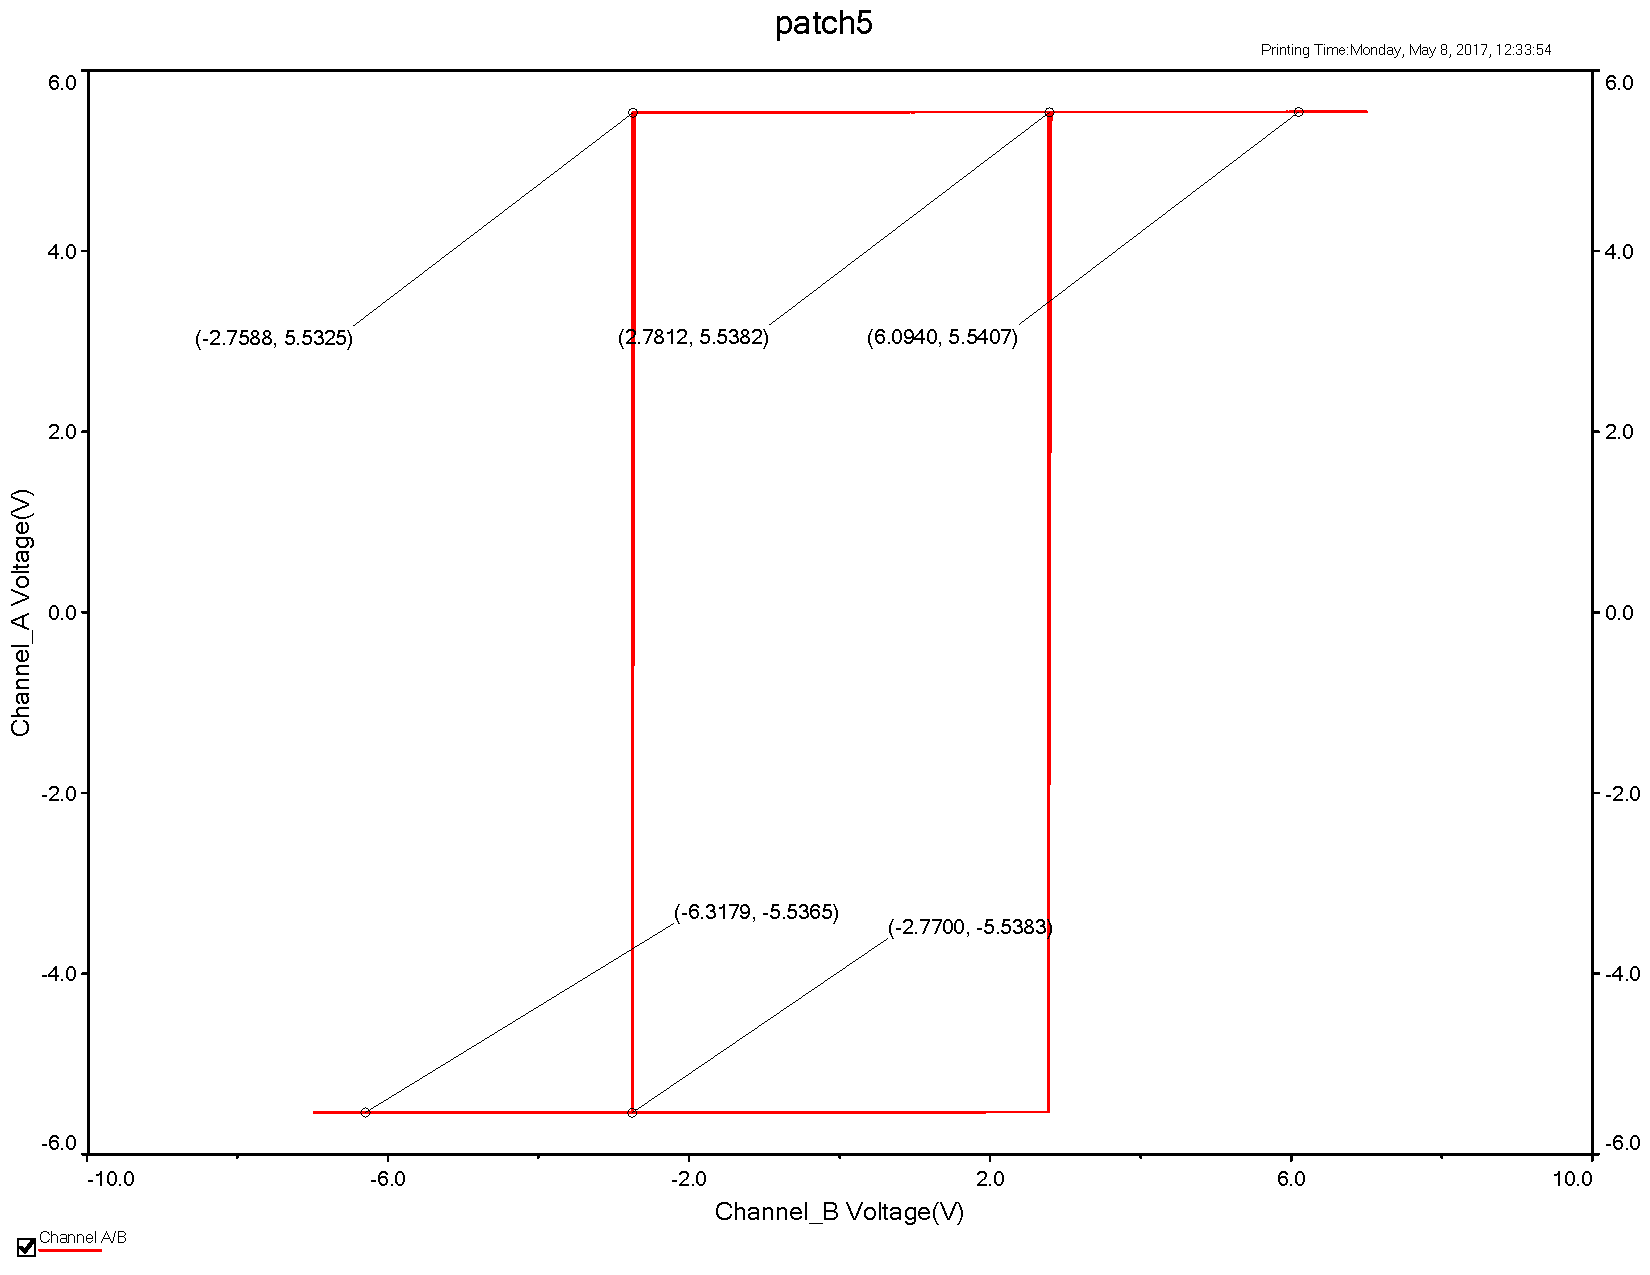
\includegraphics[width=\textwidth]{sch.pdf}
\caption{滞环特性输出波形}
\label{BI}
\end{figure}
\subsection{锯齿波发生电路}
\subsubsection{理论分析}
如图\ref{tanCrit}所示是锯齿波发生电路的测试图,根据\ref{sec:}一节的说明,我们设两个二极管的正向导通电压降为$U_D$,可以根据电路图可以得到上升和下降的方程($R_1,R_2$位置见图所示)
$$2U_T=T_-\frac{U_Z-U_D}{R_1C}$$
$$2U_T=T_+\frac{U_Z-U_D}{R_2C}$$
因此可以得到上升沿和下降沿时间
$$T_-=\frac{2U_TR_1C}{U_Z-U_D}$$
$$T_+=\frac{2U_TR_2C}{U_Z-U_D}$$
需要锯齿波下降时间为上升时间的20\%马上得到$5R_1=R_2$

同时要求电路周期不变,得到$$\frac{2U_T(R_1+R_2)C}{U_Z-U_D}=0.4\mathrm{mS}$$
可以迅速解得$R_1=5.816\mathrm{k}\Omega$,进一步得到$R_2=29.084\mathrm{k}\Omega$

具体选取$R_1=6\mathrm{k}\Omega,R_2=30\mathrm{k}\Omega$
\begin {figure}
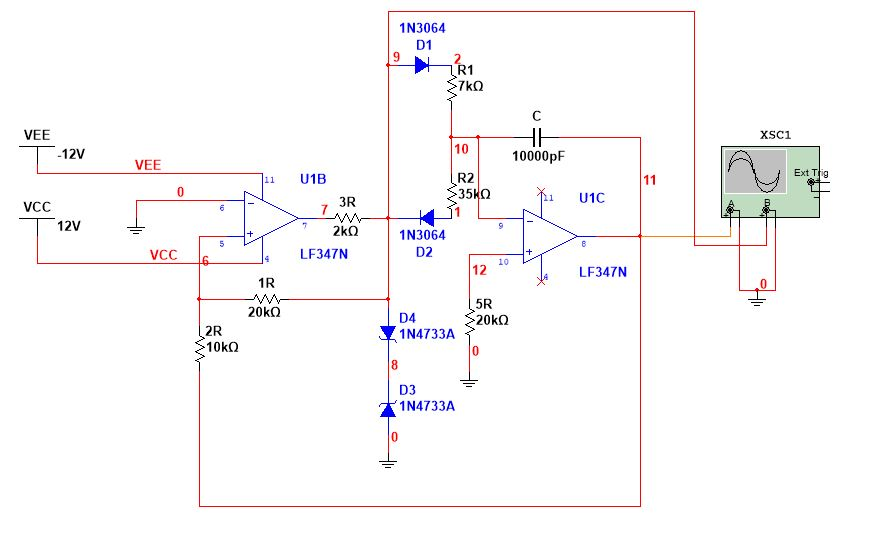
\includegraphics [width=\textwidth]{tan.jpg}
\caption{锯齿波发生电路}
\label{tanCrit}
\end {figure}
\subsubsection{输出波形仿真}
\begin{figure}
\centering
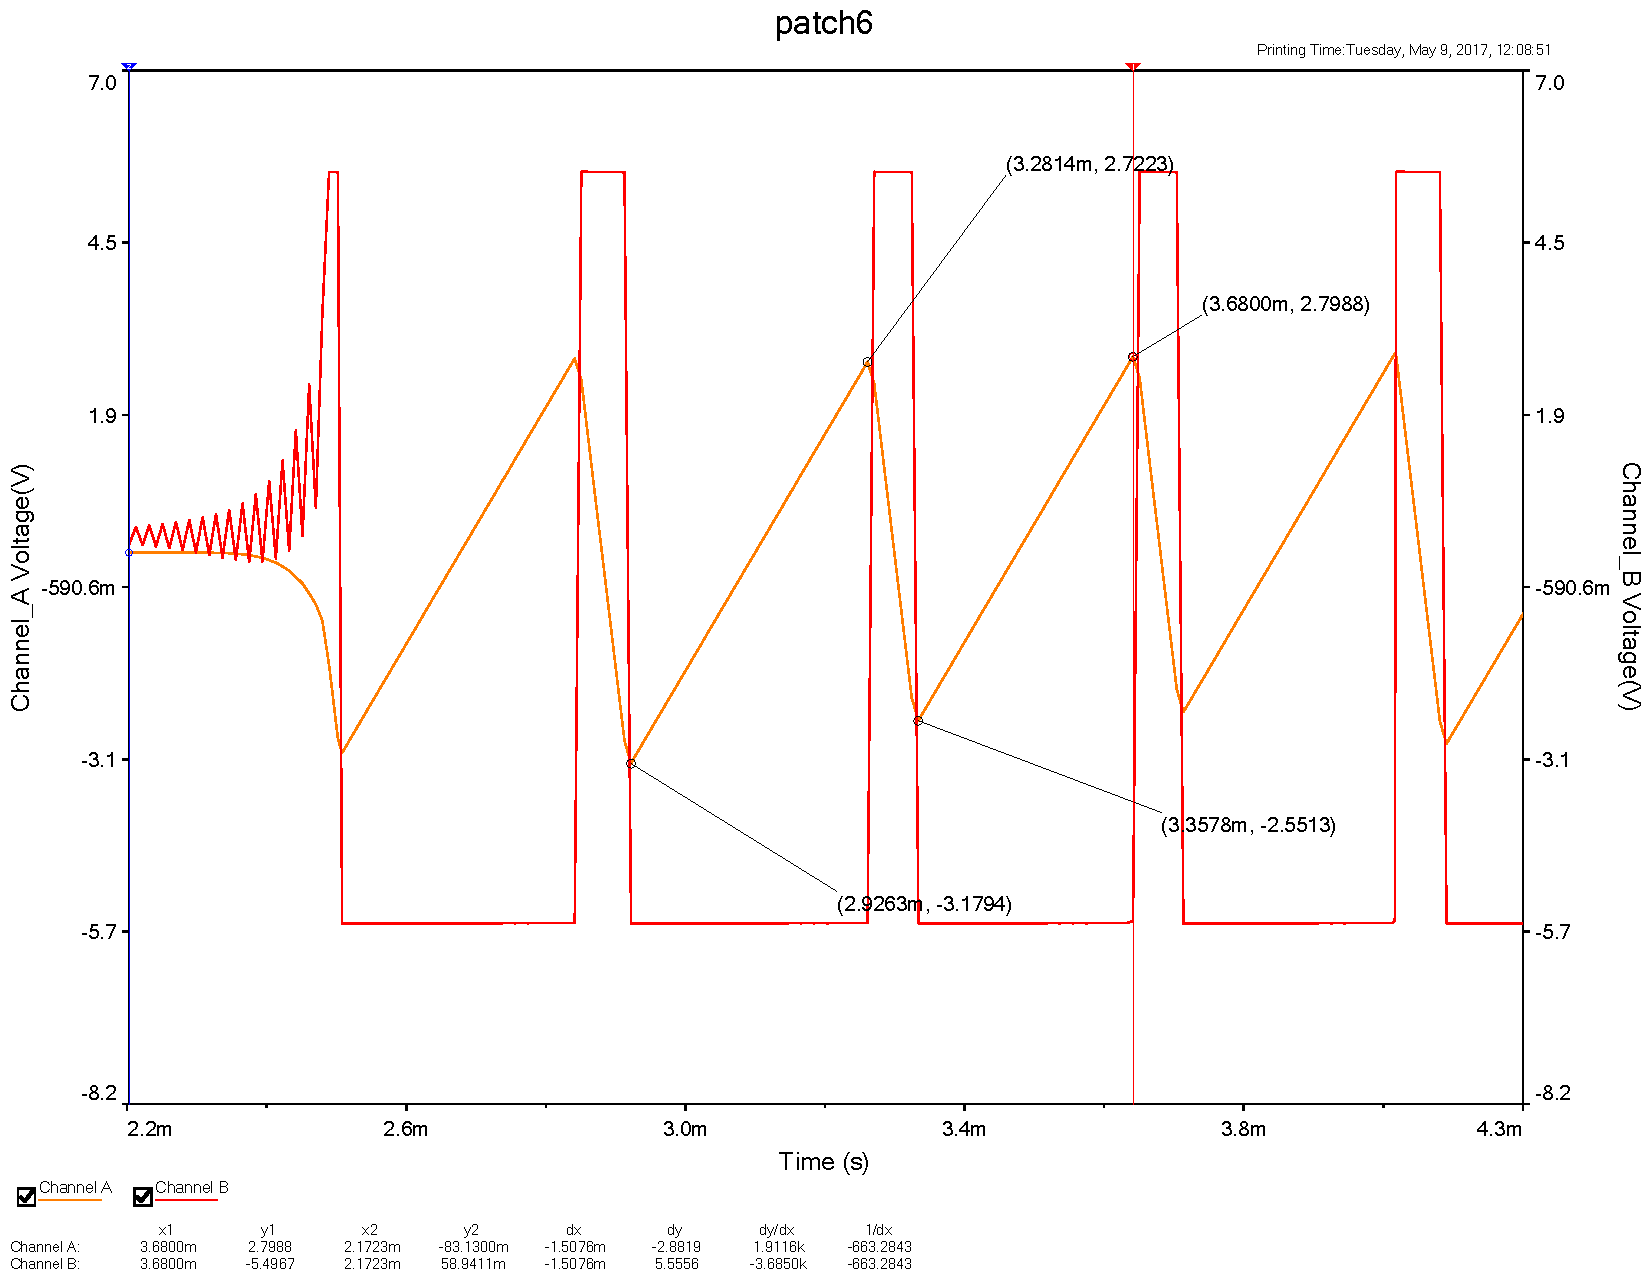
\includegraphics[width=\textwidth]{tan.pdf}
\caption{锯齿波发生电路输出波形}
\label{BI}
\end{figure}
\section{实验数据记录}
\subsection{正弦波发生电路}
\subsection{方波——三角波发生电路}
\subsection{滞环特性电路的测试}
\subsection{锯齿波发生电路}
\end{document}